\documentclass[10pt, letterpaper]{article}
\usepackage{cite}
\usepackage{fancyhdr}
\usepackage[svgnames]{xcolor}
\usepackage[colorlinks=true,
            urlcolor=black!65!white,
            linkcolor=black!65!white,
            urlcolor=black!65!white,
            citecolor=black!65!white
            ]{hyperref}
\usepackage{url}
\usepackage{tikz}
\usetikzlibrary{shapes,snakes,arrows}
\usepackage{graphicx}
\usepackage{caption}
\usepackage{subcaption}
\usepackage{listings}
\usepackage[mono]{inconsolata}

\topmargin=-5mm
\evensidemargin=0cm
\oddsidemargin=0cm
\textwidth=16cm
\textheight=22cm
\addtolength{\headheight}{1.6pt}
\hypersetup{pdfstartview=}

\tikzset{>=latex}

\newcommand{\secref}[1]{\S\ref{#1}}

\newcommand{\lastupdate}{\today}
\newcommand{\ie}{\textit{i.e.}}
\newcommand{\mdash}{---}
\newcommand{\ecall}{\textsf{ecall}}
\newcommand{\ocall}{\textsf{ocall}}
\newcommand{\env}{\textsf{environment}}
\newcommand{\mrenclave}{\textsf{mrenclave}}
\newcommand{\mrsigner}{\textsf{mrsigner}}
\newcommand{\sha}{\textsf{sha256}}
\newcommand{\pve}{\textsf{PvE}}
\newcommand{\pce}{\textsf{PcE}}
\newcommand{\qe}{\textsf{QE}}
\newcommand{\launchenclave}{\textsf{Launch Enclave}}
\newcommand{\uc}{\textsf{UC}}
\newcommand{\se}{source-enclave}
\newcommand{\te}{target-enclave}


\title{\bf Intel SGX Remote Attestation is not sufficient}
\author{\textsc{Yogesh Prem Swami}}

\date{\lastupdate}

\begin{document}
\pagenumbering{arabic}

\maketitle

\begin{abstract}
  Intel SGX enclaves provide hardware enforced confidentiality and
  integrity guarantees for running pure computations (\ie, OS-level
  side-effect-free code) in the cloud environment. In addition, SGX
  remote attestation enables enclaves to prove that a claimed enclave
  is indeed running inside a genuine SGX hardware and not some
  (adversary controlled) SGX simulator.

  Since cryptographic protocols do not compose well
  \cite{cramerthesis,ucframework,gnuc}, especially when run
  concurrently, SGX remote attestation is only a necessary
  pre-condition for securely instantiating an enclave. In practice,
  one needs to analyze all the different interacting enclaves as a
  single protocol and make sure that no sub-computation of the
  protocol can be simulated outside of the enclave. In this paper, we
  present a practical framework for analyzing enclaves. We analyze
  Intel provided EPID\cite{epid} \textsf{Provisioning} and
  \textsf{Quoting} Enclave\cite{sgxattest} within this framework and
  report our (largely positive) findings. We also provide details
  about SGX's use of EPID and report (largely negative) results about
  claimed anonymity guarantees.

\end{abstract}

\section{Introduction}
\label{sec:intro}
  Intel SGX enclaves\cite{sgxinnov, sgxinnov2} provide hardware
  enforced confidentiality and integrity guarantees for running pure
  computation (\textit{i.e.}, OS-level side-effect-free code) in the
  cloud environment. By limiting the application's Trusted Computing
  Base (TCB) to the CPU and CPU-Cache, SGX provides unprecidented
  confidentiality and integrity guarantees against malicious OS
  kernels and supervisor software. A popular design methodology---as
  evidenced by \cite{Haven, Graphene, Scone}---for creating secure
  cloud applications is as follows:

  \begin{description}
    \item[Step-1:] First, define a remote-attestation mechanism to
      securely instantiate an enclave. Quite often, this step is not
      explicitly stated probably because a generic black-box
      attestation scheme---whatever that means---is expected to be
      sufficient.
    \item[Step-2:] Then, largely independently of the
      remote-attestation mechanism, define the functionlity that needs
      to be implemented inside the enclave. This step often involves
      composing different cryptographic as well as non-cryptographic
      protocols in ad-hoc ways to implement the desired algorithm. For
      example, the enclave may need to read encypted keys from disk,
      compute a signature based on that key, create a new set of keys,
      etc.
    \item[Step-3:] Finally, define a ``run-time workflow," where one
      first validates the remote-attestation result, and then runs the
      algorithm implemented by the enclave. This step often requires
      multiple interactions with various other entities such as other
      enclaves, untrusted host software, trusted remote client
      softrware, and other cryptographic devices such as TPMs.
  \end{description}

  It's hard to argue against the simplicity and ease of implementation
  of such a modular software design. However, as pointed out in
  \cite{ucframework}, unless a protocol is desgined for
  ``\textsf{Universal Composition}" (\uc)---where, the real-world
  behavior and the ideal-world definition (function) of a protocol are
  computationally indistinguishable \textit{for every} adversary
  controlled environment---it's unlikely that arbitrary composition of
  such protocols will be secure. On the other hand, proving results in
  the \uc-framework is rather difficult. In this paper we propose a
  framework for analyzing SGX enclaves that's a compromize between a
  full \uc-based analysis and completely ad-hoc composition. Before
  describing the framework, we illustrate the problem associated with
  the protocol composition with two real-world examples.

  To set the stage, a cloud service provider\footnote{This example is
    based on a distilled version of actual protocol designed by a
    mid-sized cloud-security/compliance company.} wanted to migrate
  its new clients from Amazon Cloud-HSM to an SGX enclave. The
  protocol for interacting with the enclave was based on HTTP
  Request/Response framework, where different operations (such as
  \textsf{KeyGen}), were sent as a command, and the enclave would
  execute and return a response (including explicit error codes) back
  to the remote caller.  Important use-case for the enclave were to
  support (a) local key generation, (b) storing the public/private key
  on disk with an AEAD scheme that would allow \textit{fast}
  key-lookup, and (c) creating Certificate Signing Requests (CSR) from
  the enclave using challenge-response protocol
  \cite[\S5.2.8.3]{rfc4210}, among other
  things. Figure~\ref{fig:sequentialcomp} describes one execution path
  of the protocol.

  \begin{figure}[h]
  \centering
  \begin{subfigure}[b]{.5\textwidth}
    \centering
    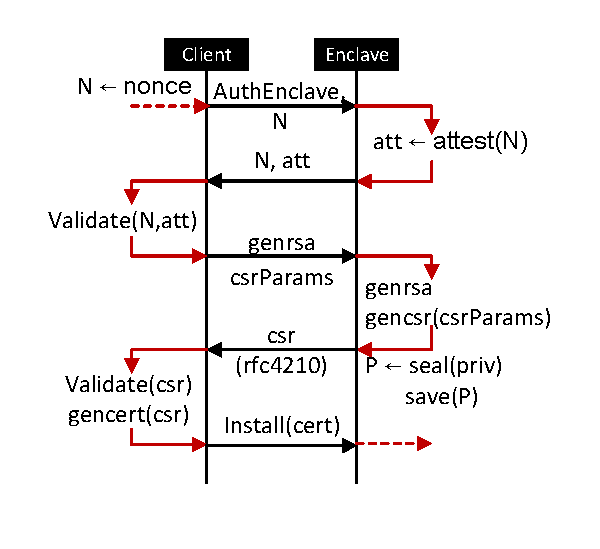
\includegraphics[width=.95\linewidth]{Diagrams/SeqCompProblem}
    \caption{Command execution for \textsf{KeyGen} with Cert}
    \label{fig:sequentialcomp}
  \end{subfigure}%
  \begin{subfigure}[b]{.5\textwidth}
    \centering
    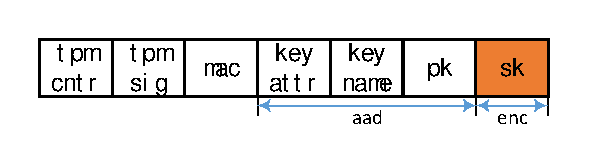
\includegraphics[width=.95\linewidth]{Diagrams/MsgFmt}\\\vfill
    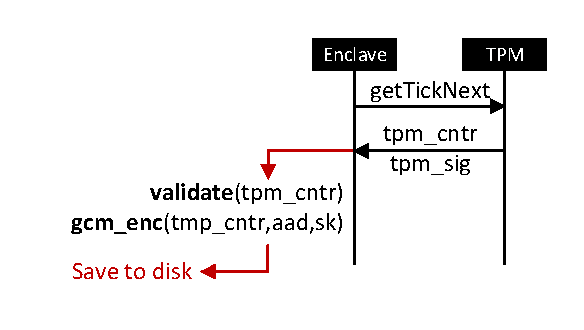
\includegraphics[width=.95\linewidth]{Diagrams/SealProtocol}
    \caption{Message format and seal protocol}
    \label{fig:sealprotocol}
  \end{subfigure}
  \caption{Example of a flawed key-management enclave. The commmand
    execution protocol ascertains the authenticity of the enclave by
    validating the EPID signature on a randomly generated 256-bit
    nonce, followed by executing an arbitrary mix of commands as
    required by the use-case. Long-term keys are stored as
    GCM-encrypted AEAD blobs. The nonce (a 32-bit counter zero-padded
    on the left to 96-bit) for each GCM record is stored in TPM, and
    the TPM returns a signature on the nonce (along with some
    additional data---to disable roll-back of TPM ``ticks.'' The
    enclave validates the TPM's signature before using the nonce for
    sealing.}
  \label{fig:usecase}
  \end{figure}

  This seemingly secure protocol is however not secure at all. Notice
  that the remote attestation in Figure~\ref{fig:sequentialcomp} does
  not prevent a malicious cloud service provider from first faithfully
  responding to remote attestation queries, but then emulate the rest
  of the protocol (including \textsf{KeyGen} and CSR) outside of the
  enclave. While this is obvious in this simplified example, in a more
  complicated scanerio, where multiple enclaves are interacting with
  each other, it might not be obvious if certain subcomponents of the
  protocol can be simulated outside. Even though the entire enclave is
  \textit{sequentially composed} from potentially provably-secure
  protocols, the combined protocol is completely insecure.

  Second, consider the seal protocol. Here each record (see
  Figure~\ref{fig:sealprotocol}) is GCM-encrypted using a nonce
  generated and signed by a TPM. However, consider a cloud service
  provider who instantiates two copies of the same enclave and
  \textit{concurrently} executes \textsf{KeyGen} using the same TPM
  signed counter. In this case, each enclave will generate two
  different keys in response to \textsf{KeyGen}. However, since the
  two concurrent instances will each correctly verify the signature
  (the two enclaves are identical), each will end up using the same
  nonce with different underlying data! As is the case with all
  counter modes, reusing the nonce can completely destroy the security
  of the system\footnote{In the present case, since the underlying
    data is uniformly distributed, at least for AES or ECDSA keys,
    such a concurrent composition might not be harmful. However, if
    there is even a small bias in the random number generator, it
    might be possible to build a distinguisher from the \texttt{xor}
    of plain-text data.}. Note that this is not a flaw in GCM or in
  the way the TPM is used\footnote{When using TPMs with SGX enclaves,
    it's important that both the TPM and the enclave mutually
    authenticate each other. Failure to do so can lead to replay
    attacks where the adversary swaps the motherboard and in doing so
    resets the TPM counter. In the present case, however, even
    mutually authenticated TPM counter might not be secure under
    concurrent composition.}, rather, it's a case where an otherwise
  secure protocol is insecure under concurrent composition.

  To summarize, \textit{an enclave is a protocol} composed of several
  sub-protocols. In order for the enclave to be secure, it's essential
  that sequential and concurrent composition of subprotocols remain
  secure. Here, by secure, it's meant that the internal state of the
  enclave cannot

  The rest of this document is organlized as follows.
  \secref{sec:model} describes the abstract computational model that's
  better suited for security ananysis. \secref{sec:analysisfwk}
  describes pitfalls of sequential, concurrent, and parallel
  composition of cryptographic protocols and describes ways in which
  an enclave can be abused by a malicious cloud service
  provider. \secref{sec:remoteatt} describes Intel's remote attestation
  framework, and describes in detail the SGX remote attestation
  mechanism.

  \section{SGX Computational Model}
  \label{sec:model}
  Intel documentation\cite{intelsdm} provides excellent low-level
  details about the SGX instructions. This section provides an
  abstract computational model of SGX which is better suited for
  security analysis of an SGX enclave.

  Abstractly, an SGX enclave can be thought of as a blackbox that's
  capable of running any arbitrary algorthim. The blackbox, hereafter
  called an enclave, communicates with the outside world, called the
  \env, in three different ways:

  \begin{figure}[h]
  \centering
  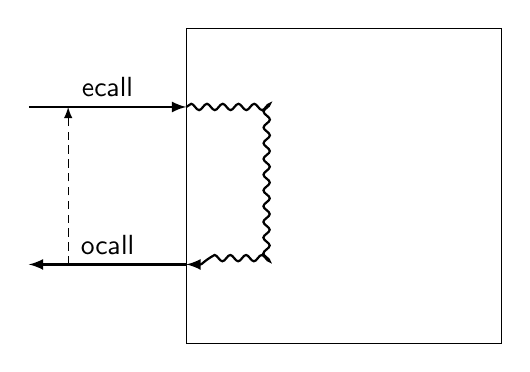
\begin{tikzpicture}[x=1cm, y=-1cm]
  \newcommand{\ench}{4cm}
  \newcommand{\encw}{4cm}
  \newcommand{\alen}{1cm}
  \newcommand{\adiff}{1cm}

  \node[rectangle, minimum height=\ench, minimum width=\encw, draw] (enc) {};
  \draw[->,thick] (-\encw / 2.0 - 2*\alen, \adiff ) -- (-\encw/2.0, \adiff) %%
  node [midway, above] {\textsf{ecall}};

  \draw [->, thick, decorate, %%
    decoration={snake,amplitude=.4mm,segment length=2mm, post length=1mm}] %%
  (-\encw/2.0, \adiff) -- (-\encw/2.0 + 1*\adiff + 0.1, \adiff) -- %%
  (-\encw/2.0 + 1*\adiff , -\adiff) -- (-\encw/2.0, -\adiff);


  \draw[<-,thick] (-\encw / 2.0 - 2*\alen, -\adiff ) -- (-\encw/2.0, -\adiff) %%
  node [midway, above] {\textsf{ocall}};

  \draw[->, thin,densely dashed] (-\encw / 2.0 - 1.5*\alen, -\adiff ) -- %%
  (-\encw/2.0 - 1.5*\alen , \adiff);
\end{tikzpicture}

  \caption{SGX Computational Model.}
  \label{fig:model}
  \end{figure}

  \begin{description}
  \item[Ecall:] The \env\ can invoke a pre-defined function inside the
    enclave by passing input parameters and returning internal state
    of the enclave as results. Such invocations from the \env\ to the
    enclave are referred to as \ecall. The parameter values passed
    from the \env\ to the enclave are either copied or directly shared
    with the enclave. An \ecall\ can terminate in one of the three
    ways: (a) by returning from the enclave, (b) by making an explicit
    \ocall, or (c) as a result of an interrupt or exception.

    SGX also supports multithreading, and it's possible for the
    \env\ to run the same \ecall\ in different threads. However, once
    an \ecall\ has acquired the thread, future attempts to reuse that
    same thread will result in error. Futhermore, the number of
    threads that an enclave can support is pre-determined by the
    enclave signer, and cannot be altered at runtime.

  \item [Ocall:] While an enclave is executing (because of some
    previous \ecall), it can make \ocall s to pre-designated functions
    in the \env.  Unlike an \ecall, an \ocall\ cannot directly share
    the internal enclave state with the \env, and must---directly or
    indirectly---copy the parameters into the \env\ before making an
    \ocall.

    An interesting characteristic of an \ocall\ is that the \env\ is
    not requred to return back to the enclave at the end of the
    \ocall\ (see Figure~\ref{fig:model}). Since the behavior of
    pre-designated functions in the \env\ are controlled by the
    adversary, one should not expect the \env\ to follow the protocol
    that enclave author envisioned. In particular, it's possible to
    create a chain of \ecall s and \ocall s such that the adversary
    can perform operations on the internal (global) state of the
    enclave.

  \item[Asynchrnonous Exit:] In addition to an \ocall, the processor
    can exit from an enclave due to an interrupt or exception. Such
    enclave exiting events are called Asynchronous Exit Events, or
    AEX. Unlike an \ocall, an AEX can transfer control from the enlave
    to the environment at arbitrary (possibly adversary controlled)
    points inside the enclave. Like \ocall s, an AEX can either by
    resumed from where the enclave left off, or the environment can
    invoke another \ecall (either within the same thread or a
    different thread).

    Since an adversary can create multiple running copies of an
    enclave and selectively interrupt each enclave to cause and AEX,
    it can be used as a means to ``rewind'' the internal state of of
    the enclave. Given that proof-of-knowledge \cite{BellarePOK}
    protocols fundamentally have a \textit{knowledge-extractor} based
    on rewinding, an enclave must ensure that it does not leak secrets
    when interrupted by an AEX.

  \end{description}

  \subsection{Enclave Creation}
  \label{sec:enclavecreateion}
  An enclave is generated as a dynamically shared library using
  standard compiler tools. In addition, the entity creating the
  enclave must also decide up-front on the following information:

  \begin{description}
  \item[Attributes:] The attributes of an enclave act as an access
    control mechanism that is enforced by the hardware. For example,
    certain high priviledge keys, such as Launch-Key and Provision-Key
    cannot be made accessible to all the enclaves, as it would
    compromize the security of entire SGX ecosystem---not just a given
    CPU. An enclave author requests the attributes needed by the
    enclave at compiler/sign time, and the Launch-Enclave, based on
    policy decisions, decides whether to grant or reject an
    authorization token (called \textsf{EINITTOKEN}) for instantiating
    the enclave.

  \item[Stack size:] The enclave author must estimate the size of the
    stack needed by enclave and set its value at enclave creation
    time. Once an enclave is instantiated, this value cannot be
    changed.

  \item[Heap size:] Like the stack size, the heap-size of the enclave
    is also fixed at enclave creation time. In SGXv2, this value can
    be changed post instantiation.

  \item[Thread count:] An enclave must also decide upon the number of
    threads that can run conconrrently. As pointed out in
    \secref{sec:model}, concurrency can have a dramatically negative
    impact on the security of the certain protocols, and one must not
    select this parameter just on the basis of performance
    requirements, but also on the basis of security concerns.

  \item[Software versioning:] SGX provides elaborate software-upgrade
    and life-cycle management faciliaties and allows software vendors
    to make use of these features.

  \end{description}

  Based on these parameters, the enclave signing tool creates a
  virtual memory layout of the enclave and computes a hash of the
  entire memory layout (including the stack, heap, thread control
  structure, etc.)  See \cite{intelsdm} for details about how the hash
  is computed. This hash, called \mrenclave, is used as the unique
  identifier for the enclave.

  In addition to \textsf{mrenclave}, the software vendor must also
  sign the enclave using a RSA-3072 key. The hash of the RSA
  Public-Key is called \mrsigner. As described in \cite{surnaming},
  the purpose of the signature is to provide an unforgeable
  identity---a \textit{surname} based lineage---to a set of enclaves
  based on the vendor.

  It should be noted that the \mrenclave\ of an enclave doesn't change
  even when the signing key is changed. This is significant when
  validating attestation or deriving keys based on \mrenclave.

  \subsection{Enclave Instantiation and Access Control}

  A properly signed enclave can be instantiated on any Intel SGX
  Processor---subject to access control restrictions enforced by
  \launchenclave. Before an enclave can be instantiated on an SGX
  capable processor, it must get an authorization token, called
  \textit{Launch Token}, from Intel provided \launchenclave. The
  \launchenclave\ uses a combination of \mrenclave, \mrsigner, the
  attributes of the enclave and a \textit{whitelist signed by Intel}
  to decide whether to grant Launch Token to the enclave or not. Once
  an enclave obtains a Launch Token, the enclave can continue using it
  indefinitely, even when the policies of the \launchenclave\ might
  get updated later on.

  \subsection{SGX Platform Keys}
  \label{ssec:platkeys}

  As described in \cite{sgxattest}, each Intel SGX capable processor
  contains two statistically independent base keys: \textit{Root
    Provisioning Key} and \textit{Root Seal Key}. The Root
  Provisioning Key is used as the Root of trust between the CPU and
  Intel Attestation Services (IAS) \cite{ias}. Intel retains a copy of
  this key at the time of manufacturing and uses it to establish the
  trustworthiness of the processor during EPID join process. Intel
  claims that Root Seal Key is not retained. However, it's not clear
  whether the this key is generated inside the processor via oracle
  access (\ie, in such a way that CPU generates the key all by itself
  using it's own internal random numbers or with PUFs), or whether the
  key is first generated outside the processor, then injected into
  CPU, and finally all outside references destroyed. Unless these keys
  are generated via oracle access, one should consider the Root Seal
  Key to be known to Intel.

  \begin{figure}
  \centering
  \begin{subfigure}[t]{.45\textwidth}
    \centering
    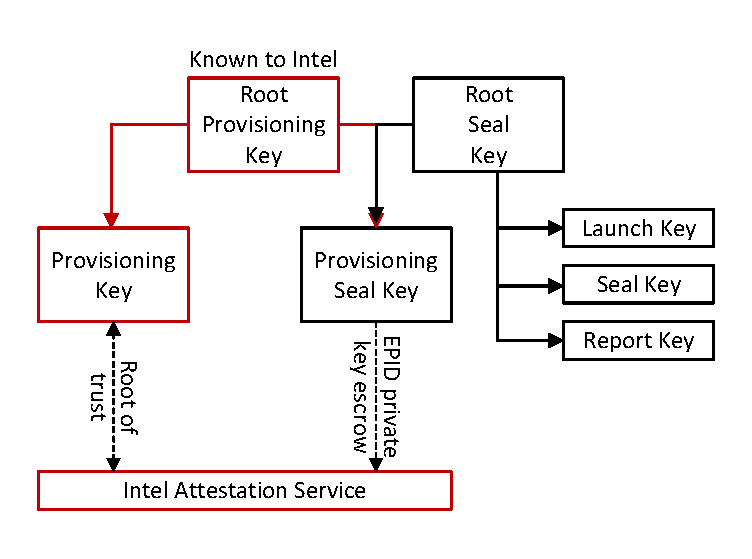
\includegraphics[width=\linewidth]{Diagrams/KeyHierarchy}
    \caption{The Provisioning Key acts as a root-of-trust between SGX
      Capable CPU and Intel Attestation Service. Provisioning Seal Key
      is used for EPID private key escrow.}
    \label{fig:keyhierarchy}
  \end{subfigure}
  \hspace{.05\textwidth}
  \begin{subfigure}[t]{.45\textwidth}
    \centering
    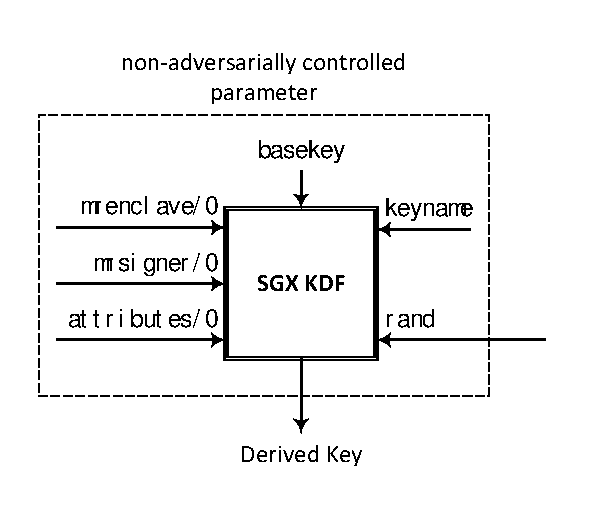
\includegraphics[width=\linewidth]{Diagrams/SGXKDF}
    \caption{SGX Key derivation function. Only parameters outside the
      dotted line can be adversarially chosen. Key derivation uses
      all-zeros for \mrenclave, \mrsigner, and attributes if keypolicy
      doesn't require them. See \cite[\S38.17]{intelsdm} for
      additional details.}
    \label{fig:sgxkdf}
  \end{subfigure}
  \caption{SGX Platform and Named Key.}
  \label{fig:keys}
  \end{figure}

  An application software does not have raw acceess to these base
  keys. However, an application can access \textit{named} keys that
  are derived from these two base key (see Figure~\ref{fig:keys}).
  The key derivation function allows enclave author to specify
  policies on how to derive enclave specific keys from base
  keys. These policies allow enclaves to use the \mrenclave,
  \mrsigner\ and/or attributes from the trusted CPU cache to derive
  keys. An implication of this design is that enclaves cannot derive
  keys that might belong to a different enclave. Also note that when
  key derivation policy does not require specific field such as
  \mrenclave\ to be used, a default value of all-zeros is
  used. Therefore, even when ``raw'' named keys are available that has
  not be specialized for any particular enclave, it's not possible to
  derive specialized keys from the raw key (assuming, of course that
  the KDF is a secure PRF). For example, one can obtain the raw
  Platform Seal Key that is neither tied to \mrenclave\ or
  \mrsigner\ of any enclave, and yet it's not possible to derive
  enclave specific Platform Seal Keys from the raw Platform Seal Key.

  The following list describes user accessible keys and their intended
  usage:

  \begin{description}
  \item[Provisioning Key:] This key is derived from Provisioning Key
    and is used as the root-of-trust between the CPU and the Intel
    Attestation Service during the EPID join process. Since admitting
    a non-SGX processor to the Intel Attesttion Service's group of SGX
    processors will completely compromize remote attestation for all
    CPUs, extreme care must be taken in granting access to
    Provisioning Key. Currently, the \launchenclave\ only grants
    Provisioning Key access to enclaves that have been signed by
    Intel. Furthermore, only Provisioning Enclave (\pve) and
    Provisioning Certification Enclave (\pce) (both created without
    debug option) have access to Provisioning Key.

  \item[Provisioning Seal Key:] This key is derived joinly from Root
    Provisioning Key and Root Seal Key. During the EPID join process,
    the EPID private-key for each platform is encrypted with this key
    and uploaded to Intel Attestation Service. (See
    \secref{ssec:epidprov} for details about EPID join process.)

    Note that the EPID private-key could not just be encrypted with
    Provisioning Key as that would destory the EPID's blinded-join
    protocol. Conversely, the EPID private-key cannot be encrypted
    just with Seal Key as that might allow non-priviledged enclaves to
    have access to EPID private key and thereby render Remote
    Attestation ineffective\footnote{If someone could access EPID
      private key---either directly, or through oracle access---they
      could sign remote attestation queries for \textit{any}
      platform. Furthermore, because of anonymimity, it will be
      difficult to determine the platform that was compromized.}.

    In spite of this design choice, given the uncertainity about how
    the Root Seal Key is generated, one should assume that Intel knows
    the EPID private key for each platform.

  \item[Launch Key:] This key is derived from Root Seal Key and is
    used by \launchenclave\ to create authorization tokens
    (\textsf{EINITTOKEN}) that each non-Intel enclave must obtain in
    order to instantiate an enclave. Only a specific \mrsigner---whose
    corresponding private-keys are only known to Intel---can access
    the Launch Key. In SGXv2, the \mrsigner\ for \launchenclave\ can
    be changed programatically, (see \cite[\S39.1.4]{intelsdm} for
    details) and any enclave signed with that \mrsigner\ can gain
    access. With this change, however, it's not clear how Intel
    intends to enforce access control restrictions on the
    Proviosioning Key.

  \item[Seal Key:] This key is derived from Root Seal Key and used for
    encrypting data specifically for a given CPU.

  \item[Report Key:] This key is derived from Root Seal Key and used
    for Local Attestation (see \secref{ssec:localatt} for detailed
    information on Local Attestation and how Report Key is used).
  \end{description}

  \subsection{Local Attestation}
  \label{ssec:localatt}



  \begin{figure}
    \centering
    \begin{subfigure}[h]{.5\textwidth}
      \centering
      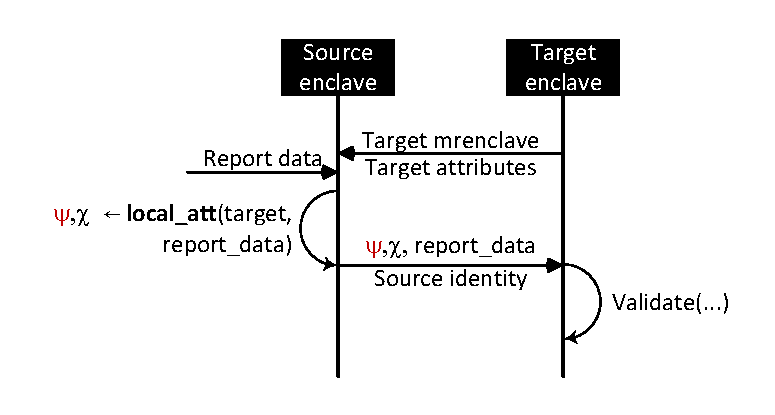
\includegraphics[width=.95\linewidth]{Diagrams/LocalAttestationFlow}
      \caption{Local attestation message flow.}
      \label{fig:localattestationflow}
    \end{subfigure}%
    \begin{subfigure}[h]{.5\textwidth}
      \centering
      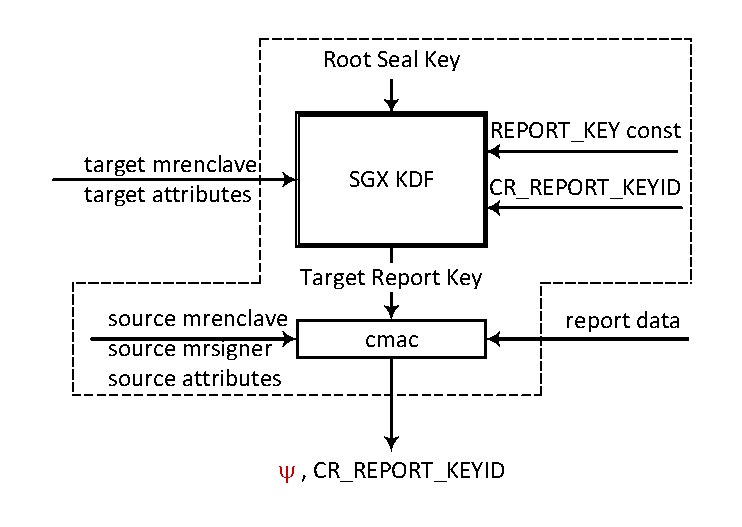
\includegraphics[width=.85\linewidth]{Diagrams/LocalAttestation}
      \caption{Local attestation computation. Parameters outside the
        dotted line can be adversarially selected.}
      \label{fig:localattestation}
    \end{subfigure}%
    \caption{Local attestation computation and message flow}
    \label{fig:localatt}
  \end{figure}

  The process of local-attestation allows a source enclave (\se) to
  prove to a target enclave (\te)---running locally on the same
  platform---that the \se\ is indeed running on a genuine Intel SGX
  platform (see Figure~\ref{fig:localattestationflow}). In addition,
  the \se\ can optionally use 512-bits of additional data (e.g., hash
  of public-key), called report-data, to claim knowledge of certain
  bit-string.

  The process of local-attestation involves computing CMAC
  \cite{aescmac} on the \se's identity (i.e., \mrenclave, \mrsigner,
  etc.) using the \te's Report Key. However, as pointed out in
  \secref{ssec:platkeys}, the \se\ cannot directly access \te's Report
  Key. SGX solves this problem by providing \textit{oracle access} to
  \te's Report Key via \textsf{EREPORT} instruction
  \cite[\S14.4.1]{intelsdm}. To compute local attestation, the
  \se\ obtains the \mrenclave\ and attributes of the \te\ through some
  out-of-band mechanism (which might be adversarial). Based on \te's
  \mrenclave, the \textsf{EREPORT} instruction internally derives the
  \te's Report Key and computes \textsf{CMAC} on \se's \mrenclave,
  \mrsigner, and attributes from the trusted CPU cache (and optionally
  untrusted user data).  The \textsf{EREPORT} instruction also uses a
  boot-time random number called \textsf{CR\_REPORT\_KEYID} to
  diversify the \te's Report Key before \textsf{CMAC} computation. The
  \textsf{EREPORT} instruction also returns the value of
  \textsf{CR\_REPORT\_KEYID} that was used during \te's Report Key
  derivation.

  The verifiation of local attestation involves using \textsf{EGETKEY}
  instruction to fetch the \te's Report Key and validating the
  \textsf{CMAC} on Report body in software.  The report body includes
  \mrsigner, \mrenclave, attributes, and other paramters of the
  \se. Note that while fetching the report key for verification, the
  \textsf{EGETKEY} will requite the value of
  \textsf{CR\_REPORT\_KEYID} to derive the right Report Key.

  \section{Enclave malleability and Knowledge Extractors}
  \label{sec:analysisfwk}

  Given the computational model of SGX, we describe certain pitfalls
  in enclave design that might inadvertantly make the enclave
  malleable, or open door for building knowledge-extractors
  \cite{BellarePOK}.

  \subsection{Enclave malleability}
  \label{ssec:malleability}
  As described in \secref{sec:model}, an application can exit an
  enclave either via (a) as a function return from an \ecall\ (b) as
  an \ocall\ or (b) as an AEX. Since it's not required for an
  \ocall\ or AEX to return back to the enclave from the state it left
  off, it's possible for a malicious \env\ to make unexpected \ecall s
  to alter the internale state of the enclave. Enclaves whose global
  internal state can be influenced by an attacker by not following the
  expected protocol are called \textit{malleable enclaves} in this
  document.

  To better understand enclave malleability, consider the following
  example: The US govenment wants to use an SGX enclave to implement
  2-man rule for launcing nuclear messiles. The 2-man rule requires
  that at least two \textit{different} members (generals) of the armed
  forces must authorize the enclave before it can launch a nuclear
  missile.

  Listing~\ref{code:malleability} describes one way to implement this.
  Essentially, the enclave keeps a list of generals, their
  public-keys, and their individual authorization state in a global
  variable \texttt{GENERALS}. In addition, the enclave keeps the
  number of distinct generals who have authorized the launch in a
  global variable \texttt{auth\_count}. Since different generals might
  be authorizing the launch at different times, the enclave allows
  each general to authorize a launch individually by signing the
  concatenation of general's name and some auxilary data.

  \begin{center}
  \lstset{language=C++,
          numbers=left, numberstyle=\tiny,
          numbersep=5pt, stepnumber=1,
          emph={auth_and_launch,auth_count},
          emphstyle=\color{red!80!black},
          emph={[2]valid_general},
          emphstyle={[2]\color{green!40!black}},
          basicstyle=\ttfamily,
          keywordstyle=\color{blue}\ttfamily,
          stringstyle=\color{red}\ttfamily,
          commentstyle=\color{brown}\ttfamily,
          morecomment=[l][\color{magenta}]{\#}
  }
  \begin{lstlisting}[captionpos=b,
                     caption={An enclave suseptible to state malleability},
                     label=code:malleability]
/* count of generals who have authorized launch. */
static int auth_count = 0;

/* hardcoded list of generals and their PKs      */
struct general_info{
  char                     general_name[256];
  const sgx_ec256_public_t general_pub;
  bool                     has_authorized; // initialized to false
}GENERALS[] = { ... };

/* ecall made by each general with a sig on name + aux data */
int auth_and_launch(const char* const general_name,
                    const sgx_ec256_signature_t* sig){
  struct general_info* valid_general = validate_general(general_name, sig);

  if(!valid_general){ return INVALID_GENERAL; }

  if(!valid_general->has_authorized){
    auth_count++; // AEX here will be devastating!
    valid_general->has_authorized = true;
  }else{
    return GENERAL_ALREADY_AUTHORIZED_ACTION; // replay
  }

  if(auth_count == 2){
    return nuke_the_kashbah(location);
  }

  return PENDING_AUTHORIZATION;
}
\end{lstlisting}
\end{center}

  Can this enclave be exploited to launch a missile with \textit{just
    one} authorization, say $\langle g_1, \sigma_1 \rangle$?
  Surprisingly, the answer is yes! Here is how:

  \begin{enumerate}
  \item The attacker first feeds $\langle g_1, \sigma_1 \rangle$ to
    \texttt{auth\_and\_launch} function with the intent of causing an
    AEX between lines 19 and 20. Since the attacker can artificially
    cause an interrupt and also instantiate multiple copies of the
    enclave in parallel, given a polynimial number of trials (in
    program length), the attacker can cause an AEX between line 19 and
    20 W.H.P. Note that at the time of a successful AEX between line
    19 and 20, the \texttt{auth\_count} and \texttt{has\_authorized}
    variables will be in an inconsistent state where the
    \texttt{has\_authorized} would still be \texttt{false} and another
    \ecall\ to \texttt{auth\_and\_launch} will successfully update the
    \texttt{auth\_count} variable.

  \item After the enclave has been interrupted by AEX and the
    processor is ready to resume, the attacker instead of resuming,
    makes an \ecall\ to \texttt{auth\_and\_launch} again with the same
    old parameters $\langle g_1, \sigma_1 \rangle$. Since the first
    \ecall\ had incremented the counter, but left the authorization
    state inconsitent, the second \ecall\ will once again increment
    \texttt{auth\_count} leading to a nuclear attack!

  \item While not applicable in this case, in some cases it might be
    necessary for an attacker to resume the first \ecall\ after the
    second one has completed. Since the enclave preserves the stack
    before making an AEX, resuming the first \ecall\ tantamouts to
    executing \textsf{ERESUME} assembly instruction.

  \end{enumerate}

  It should be emphasized that the problem of state-malleability,
  where the attacker can influence the internal state of the enclave
  without ever having direct authorized access to it, is broader in
  scope than the race condition described above. For example, one can
  use malleability to induce an error which turns the enclave into an
  oracle. It should also be emphasized that enclaves should return
  error codes with security consideration in mind.

  \subsection{Enclave rewinding and knowledge-extractors}
  \label{ssec:rewind}

  Zero-Knowledge Proof of Knowledge (ZKPK) protocols, by definition
  have in-built knowledge-extractor \cite{BellarePOK, maurerZKP}.
  Normally, the knowledge-extractor from the prover is designed by
  giving a simulator the capability to ``rewind'' the prover's state
  to arbitrary point during it's execution. Since SGX enclaves can be
  interrupted by an AEX, it's imporant that a malicious \env\ is not
  able to rewind the enclave in such a way that it inadvertantly
  reveals the secret-key.

  Consider the three-move---commit, challenge,
  blinded-reveal---$\Sigma$-protocols \cite{sigmaprotocol} that are
  the most efficient and widely-used ZKPKs protocol in practice.
  Normally, one designs $\Sigma$-protocols \textit{with interaction}
  between a prover and a verifier in mind, and then uses Fiat-Shamir
  \cite{FiatShamir} heuristic\footnote{In the Fiat-Shamir heuristic,
    the prover \textit{pretends} to be a verifier and a random oracle,
    based on publically known fields of the protocol (such as the
    commitment value, user's input message, etc.) generates the
    challenge string.} to convert it into a useful non-interactive
  use-case such as a signature scheme. Most of these protocols just
  require the prover, which in this case will be enclave, to respond
  to two challenege message for a given commitment message to reveal
  the secret.

  If an enclave is not implemented appropriately, one can induce an
  artificial AEX right after the commitment phase, and call the
  enclave with different messages in possibly different threads to
  generate two responses to the same commitment message. Note that AEX
  in conjunction with multithreading opens doors for a limited form of
  enclave rewinding and presents a larger attack surface than AEX
  alone.  Unless, an enclave requires multithreading, it's wise to set
  the number of possible threads to the bare minimum.

  \section{SGX remote attestation}
  \label{sec:remoteatt}

  SGX is an example of a hardware/software co-design of a
  cryptographic platform. A common concern in the design of such
  systems is to ensure that an adversary is not able to switch the
  hardware with a software simulator (such as QEMU \cite{qemu,
    opensgx}) of the hardware. Since an Universal Turing Machine can
  simulate any piece of computing hardware, unless there's an inbuilt
  asymmetry between what the software ``knows'' and what the hardware
  knows, it's impossible to prevent software simulator attacks in such
  systems. On the other hand, each idependent piece of software needs
  to prove on its own that it's running on a real hardware.
  Therefore, each independent software must somehow have direct or
  oracle access to the secret that the hardware is holding. The
  essence of any remote-attestation scheme in such systems is to
  address these two conflicting requirements. {\em Note}: Even limiting
  access to raw hardware keys via an oracle is not sufficient to thwart
  simulator based attacks. An attacker can run it's hardware simulator
  on a real hardware, gain access to the hardware-secret via the
  oracle, and then impersonate as the real hardware.

  In case of Intel SGX, the question of knowledge-asymmetry between
  hardware and software is answered by the Root Provisioning Key (see
  \secref{ssec:platkeys}). The dilemma of both denying as well as
  granting access to this hardware secret is soved by a two-step
  process:

  \begin{enumerate}
    \item Intel has created a (set of) priviledged enclaves---called
      \textsf{Provisioning Enclave} (\pve) and \textsf{Provisioning
        Certification Enclave} (\pce)\footnote{Intel addresses these
        enclaves by their acronyms, \pve\ and \pce, only. The
        descriptive names are author's interpretation.}---with raw
      access to the Provisioning Key and Provisioning Seal Key. The
      \pve\ and \pce\ use the Provisioning Key as the root-of-trust
      between Intel Attestation Service and the SGX CPU to bootstrap a
      new set of credentials for a Group Signature Scheme called
      Enhanced Privacy ID (EPID) \cite{epid}. Since EPID key
      provisioning takes place only once\footnote{EPID re-provisioning
        might take place if the CPU's Security Version Number (CSVN
        \cite[\S39.4.2.2]{intelsdm}) or the Software Version Number
        (ISVSVN \cite[\S39.4.2.1]{intelsdm}) of \pce\ changes.}, the
      Provisioning Key has minimal exposure.

    \item Once a platform has been provisioned with EPID keys, another
      Intel signed enclave called \textsf{Quoting Enclave} (\qe) is
      given raw access to EPID keys and made responsible for
      generating remote-attestation results on behalf of other
      arbirary--potentially malicious---enclaves.

      To compute remote attestation, an arbitrary enclave first
      generates a local attestation with \textsf{Quoting Enclave} as
      the target enclave in Figure~\ref{fig:localattestationflow}. The
      \textsf{Quoting Enclave} first validates the local-attestation
      report and subsequently uses EPID key to sign all the parameters
      it validated during local attestation. Since local-attestation
      uses the hardware resident identity of the enclave (i.e.,
      \mrenclave, \mrsigner, and enclave attributes), which canot be
      forged (see \secref{ssec:localatt}), the remote-attestation
      result on the enclave identity cannot be forged
      either. Furthermore, since arbitrary software never has direct
      or oracle access to either Provisioning Key or EPID
      private-keys, simulator based attacks where the simulator itself
      is a valid enclave are also thwarted.
  \end{enumerate}

  Remote attestation is a crucial component in the overall design of
  SGX platform. While local-attestation (see \secref{ssec:localatt})
  uses a MAC (CMAC), whose properties are well-known and widely
  studied, SGX remote-attestation is based on a Group Signature Scheme
  \cite{ChaumGroupSignatures} called Enhanced Privay ID
  (EPID)\footnote{Unfortunately, the way Intel has implemented remote
    attestation, this statement is only partially correct. While the
    underlying scheme is based on EPID, the quoting enclave---which is
    responsible for generating the group signature also
    \textit{encrypts each signature} with an authenticated public-key!
    Since no-one apart from Intel can decryt these signatures, no
    one---not even those with access to Group Public-Key--can validate
    these signatures.} \cite{epid}. Even though group signatures have
  been studied for a long time \cite{camenischLysyankaya,
    coalitionresistant, BMW03, dynamicGroupSignatures}, it wasn't
  until the Trusted Computing Group decided to use Direct Anonymous
  Attestation (DAA) \cite{daa} that they became widely used. In spite
  of this long history, until very recently DAA was known to have
  well-known, serious, real-world \cite{tpmDHOracle}, cryptographic
  flaws \cite{daaproblems} in widely deployed systems. It's only
  recently that a unified security model has been proposed
  \cite{ucdaa} and proven correct in \uc\ framework. It's therefore
  crucial to analyze EPID as a signature scheme as well as Intel's
  implementation to have confidence in the remote attestation
  mechanism.

  The rest of this section is organized as follows: \secref{ssec:epid}
  provides a bird's eye view of Group Signatures and EPID security
  model. Readers faimilar with Group Signatures, EPID, or DAA can
  safely skip this sub-section. \secref{ssec:pairings} provides
  implementation details about the Pairings Group used by Intel's
  \textsf{Provisioning Enclave} and \textsf{Quoting
    Enclave}. \secref{ssec:epidprov} provides detailed information on
  how the \textsf{Provisioning Enclave} joins the Intel SGX EPID
  group. Finally, \secref{ssec:qe} provides details about
  \textsf{Quoting Enclave} and how SGX remote attestation should be
  validated against Intel Attestation Service.

  \subsection{EPID Overview}
  \label{ssec:epid}
  In a standard signature scheme, such as ECDSA or RSA-PSS, each
  signer has a unique private/public key-pair. Given two
  message/signature pairs $\langle m_1, \sigma_1 \rangle$ and $\langle
  m_2, \sigma_2 \rangle$, an attacker in possession of $N$ public-keys
  can easily determine if $m_1$ and $m_2$ were signed by the same
  private key or not. If such signatures are generated by physical
  devices, it can be used to track the signing device and thereby
  destroy the anonymity and privacy of the person using that device.

  Group Signatures were introduced by Chaum and Van Heyst
  \cite{ChaumGroupSignatures} as a means to preserve the
  unforgeability and non-repudiation (in case of a dispute) of a
  standard signature scheme, without compromizing the anonymity of the
  signer. 

  \cite{bbs}
  \cite{bbsplus}
  \cite{concurrentJoinGroupSignatures}

  \subsection{SGX Pairing Groups}
  \label{ssec:pairings}

  \subsection{SGX EPID provisioning}
  \label{ssec:epidprov}

  \begin{figure}
  \centering
  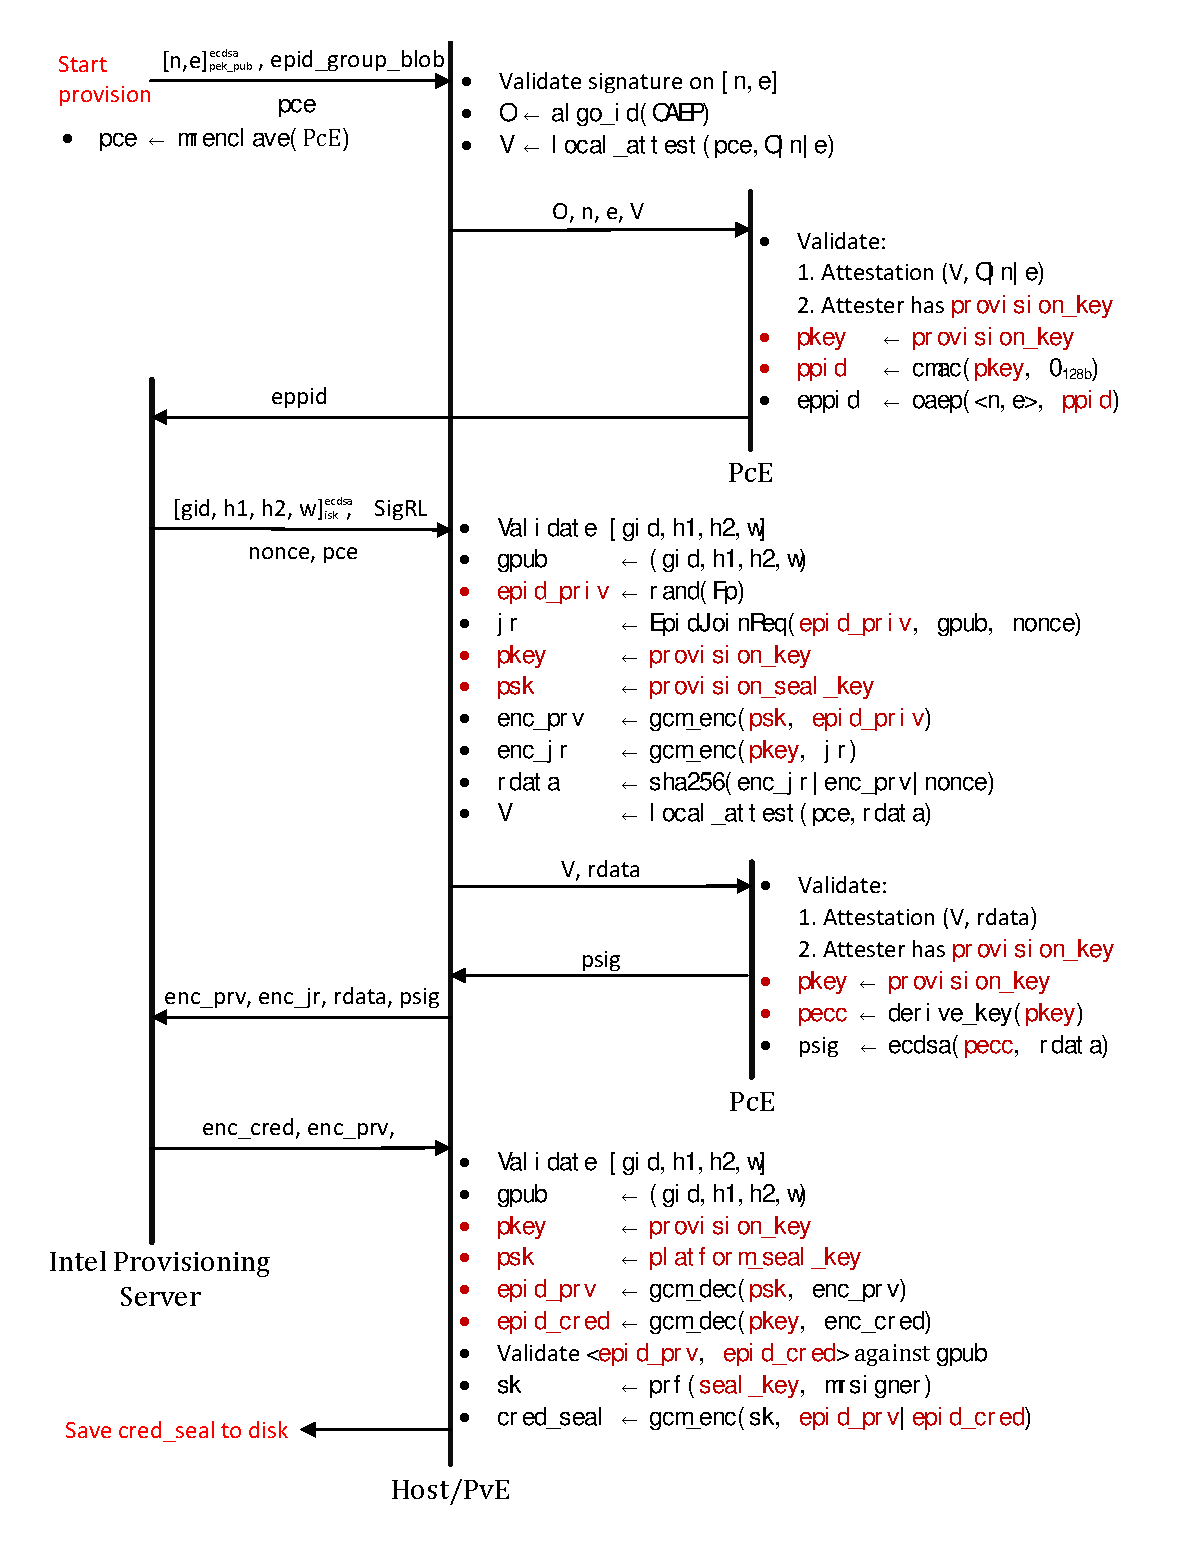
\includegraphics[width=0.8\linewidth]{Diagrams/EpidProvisioning}
  \caption{Local attestation computation. Parameters outside the
    dotted line can be adversarially selected.}
  \label{fig:epidprov}
  \end{figure}

  \subsection{SGX Quoting Enclave and Quote Validation}
  \label{ssec:qe}

  \section{Conclusion}
  \label{sec:conclusion}

\bibliographystyle{alpha}
\bibliography{sgx_biblio}

\end{document}
